%!TEX root = ../../super_main.tex

\section{Compression}
\label{sec:compression}

As described in \secref{sec:general_strategies}, we would like keep the power consumption of our application low. One way of doing this is ensuring that the amount of data sent from our application to our server is the minimum amount necessary, because sending less data costs less power and thereby also less money. During the development we discovered that many of the data types used for sensor measurements have significant overhead, compared to what is necessary in order to store the data, which opens up for the possibility of compressing the data. 
\\\\
An example of this is the heart rate sensor in the Microsoft Band 2 wearable, which uses an signed integer in order to store a heart rate. A signed integer is typically 32 bits, and has a maximum value of $2^{31} - 1$ (2,147,483,647), while a heart rate over 250 is very abnormal. This knowledge would allow us to exploit the limited value range, and use as little as 8-10 bits (values 255-1023). This would effectively cut off the majority of bits used to store a value. Furthermore, Microsoft Band 2 also uses a boolean to represent if the reading is precise (they call it locked), which uses 8 bits. This effectively means that even if you use 10 bits for the heart rate, and 1 for the locked state, you would still save 29 bits.    
\\\\
There are many more cases like that in the sensor readings, and we decided to implement a strategy for compressing one of the common values returned by many sensors, namely an array of floats containing three values. An example of a sensor that returns such measurements is the accelerometer which measures how the phone moves on its $x$, $y$, and $z$ axes. We designed a class called \mono{FloatTripleMeasurement} which is used to compress these three values to a single \mono{long}, meaning we convert $12$ bytes ($3$ floats $\times 4$ bytes) to be stored in $8$ bytes. We do this by sacrificing some of the precision of a regular float, because we think the regular precision is overkill, both in terms of sensor inaccuracy and also its usefulness for the customers. When compressing, we assume that the integer part (of the float) does not exceed $7$ numbers. We do this because the sensors only produce values ranging from $-360$ to $360$. We strip the decimal separator from the floats and treat them as a $20$ bit integer value, where the first bit determines whether the value is positive or negative. This means that we now use $60$ bits for storing the compressed value of the floats. We use the remainder of the long to add 3 bits for representing where the decimal should be placed. A visualization of the method used to compress floats can be seen in \figref{fig:float_triple_convert} and \figref{fig:float_triple_bit} respectively.

\begin{figure}[!htbp]
    \begin{alignat*}{6}
       &8.138   &&                   &&   && 8138  &&                   && \text{\mono{00000001111111001010}} \\
      -&12.821  && ~~ \rightarrow ~~ && - && 12821 && ~~ \rightarrow ~~ && \text{\mono{10000011001000010101}} \\
       &42.4878 &&                   &&   && 42487 &&                   && \text{\mono{00001010010111110111}} 
    \end{alignat*}
    \caption{Compression of floats.}
    \label{fig:float_triple_convert}
\end{figure}
\FloatBarrier

\begin{figure}[!htbp]
    \centering
    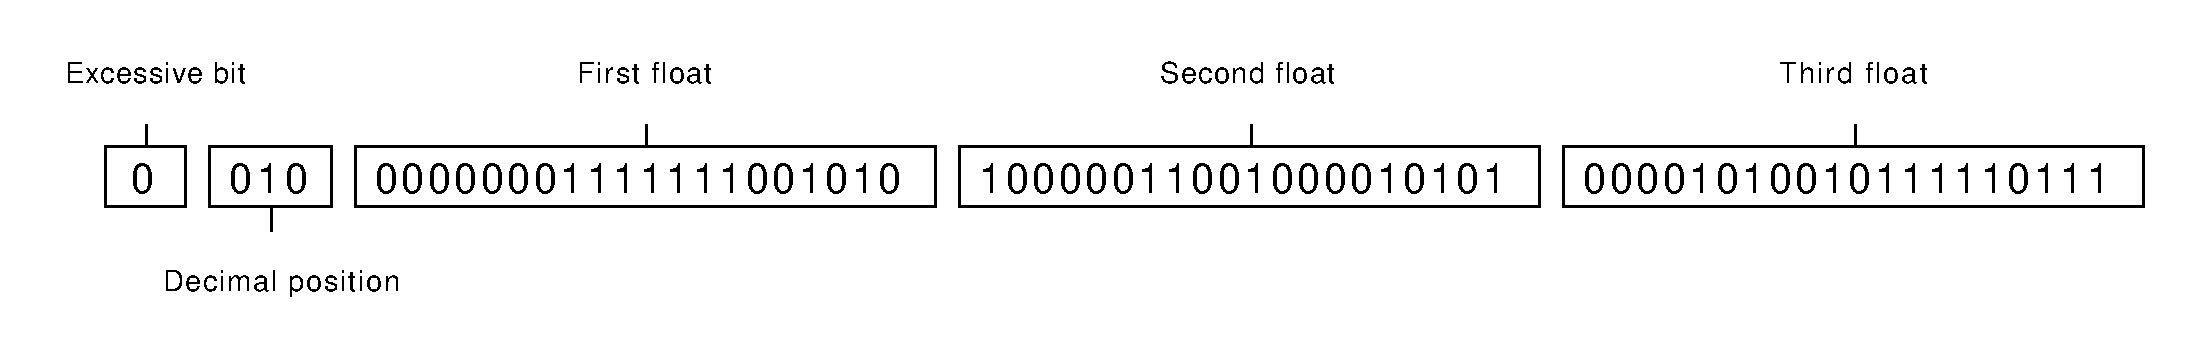
\includegraphics[width=\textwidth]{graphic/gathering_sensor_data/float_triple_bit}
    \caption{The bit representation of a \mono{FloatTripleMeasurement}.}
    \label{fig:float_triple_bit}
\end{figure}
\FloatBarrier

We wanted to compress the floating point values of the sensors so that the size of the data we need to send over network and store on the device would decrease. However, this compression does not come for free. We actively make a trade off between size of data stored and CPU cycles used for compressing and decompressing the values. We have conducted a performance test for our compression of floats that investigates how much extra time has to be spent on compressing and decompressing the floats. In the test we create a number of arrays that each contain three float values. The actual test is how fast the three float values can be multiplied together. We do this in two ways: One where we compress and decompress the float values first, and another one where we just multiply. This can give us an indication of how much time is lost on the compression when performing another task. The results of the test can be seen in \tabref{tab:results_of_compression_test}.

\begin{table}[!htbp]
\centering
    \resizebox{\textwidth}{!}{%
        \begin{tabular}{|l|l|l|l|l|l|l|}
            \hline
            ~ & \multicolumn{3}{|c|}{1+ One} & \multicolumn{3}{|c|}{Nexus 5 } \\ \hline
            Count    & \begin{tabular}[c]{@{}l@{}}With \\ compression\end{tabular}  & \begin{tabular}[c]{@{}l@{}}Without\\ compression\end{tabular} & Ratio & \begin{tabular}[c]{@{}l@{}}With \\ compression\end{tabular}   & \begin{tabular}[c]{@{}l@{}}Without \\ compression\end{tabular} & Ratio \\ \hline
            10000   &   83 ms   &   11 ms   & 7.55  &   77 ms   &   10 ms   & 7,70  \\ \hline
            100000  &  635 ms   &  172 ms   & 3.69  &  783 ms   &  113 ms   & 6,93  \\ \hline
            1000000 & 9088 ms   & 1333 ms   & 6.82  & 8245 ms   & 1090 ms   & 7,56  \\ \hline
        \end{tabular}%
    }
    \caption{Results of compression test}
    \label{tab:results_of_compression_test}
\end{table}
\FloatBarrier

As can be seen in \tabref{tab:results_of_compression_test}, it generally took seven to eight times as long to perform the multiplication when we used compression and decompression. It is, based on these results, pretty obvious that rather many CPU cycles will have to be spent on this. With this in mind, one has to consider if these extra CPU cycles, extra battery usage, etc, is worth the tradeoff. On one hand, it is possible to spend additional CPU cycles, and thereby power, before storing data on the device, in order to save $\sim 33\%$ of the space, while having to transfer less data to the server and thereby spending less power and CPU cycles on this. On the other hand we could save all the power before storing, just save the normal floats in the database, and then have to spend extra power for transferring because there is simply more data. We do not know if our approach uses more power than simply not doing it, but if the system should be expanded into something large scale, it should definitely be tested. One thing that we can definitely know for sure is that our approach uses less disk space, which is also something to consider. 
\\\\
There are furthermore the considerations of how modern compression algorithms will handle our single long compared to the three floats. In Android the standard class for sending HTTP requests automatically compresses requests to a format called gzip. To see if this compression would further reduce the space of the collection information, we conducted a small test, where we compressed (using gzip) some snapshots containing \mono{FloatTripleMeasurement}s, and compared them to compressed (also using gzip) snapshots containing regular floats. Note that both the snapshots were serialized using JSON, similar to what is outputted by the server, as seen in \lstref{lst:snapshot_json_example}. When compression with gzip, you may specify how fast the algorithm should perform the compression. The faster you specify, the less compression would be achieved. We conducted a test where we would compress using the \mono{fast} setting, but also the \mono{best} setting (slowest). The result of the conducted test can be seen in \tabref{tab:gzip_compression}. All sizes are measured in bytes.

\begin{table}[!htbp]
\centering
\begin{tabular}{r|l|l|l|}
\cline{2-4}
                                                                           & \textbf{No gzip} & \textbf{Fast gzip} & \textbf{Best gzip} \\ \hline
\multicolumn{1}{|r|}{\textbf{Size with \mono{FloatTripleMeasurements}}}    & 101,543          & 40,532             & 38,358             \\ \hline
\multicolumn{1}{|r|}{\textbf{Size with regular float measurements}}        & 118,660          & 44,893             & 38,643             \\ \hline
\multicolumn{1}{|r|}{\textbf{Difference}}                                  & 17,117           & 4,361              & 285                \\ \hline
\end{tabular}
\caption{gzip float compression test result. All sizes are in bytes.}
\label{tab:gzip_compression}
\end{table}
\FloatBarrier

This test indicates, as expected, that the biggest size difference is when not using gzip. However, when using the \mono{fast} setting, gzip will further compress the data to $\sim 38-40\%$ of the original size, and here we still see a $\sim 10\%$ difference in the size of two snapshots, indicating that using both compression methods would yield a noticeable result. When using the \mono{best} setting, the data is compressed to $\sim 33-38\%$ of the original size, however, here there is not a big difference ($\sim 1\%$) between the two snapshots, indicating that if we use the \mono{best} setting, we would not gain too much in term of size.  
